%%===========================================================%%
%%                                                           %%
%%                    RP EFFICIENCY APPENDIX                 %%
%%                                                           %%
%%===========================================================%%

\chapter{RP efficiency}\label{appendix:rpEff}

\section{RP track acceptance, reconstruction and selection efficiency}
%--------------------------- 
\begin{figure}[hb]
\caption[RP track acceptance, reconstruction and selection efficiency on the east (MC embedded into zero-bias data).]{RP track acceptance, reconstruction and selection efficiency on the east side obtained from MC simulation embedded into zero-bias data. Each plot corresponds to $z$-vertex range given in the plot.}\label{fig:rpEffE}
\centering
\parbox{0.495\textwidth}{
  \centering
  \includegraphics[width=\linewidth,page=3]{graphics/corrections/mcFullEffPxPy.pdf}\\
  \includegraphics[width=\linewidth,page=5]{graphics/corrections/mcFullEffPxPy.pdf}
}~
\parbox{0.495\textwidth}{
  \centering
  \includegraphics[width=\linewidth,page=4]{graphics/corrections/mcFullEffPxPy.pdf}\\
  \includegraphics[width=\linewidth,page=6]{graphics/corrections/mcFullEffPxPy.pdf}
}%
\end{figure}%
\begin{figure}[hb]\ContinuedFloat
\centering
\parbox{0.495\textwidth}{
  \centering
  \includegraphics[width=\linewidth,page=7]{graphics/corrections/mcFullEffPxPy.pdf}\\
  \includegraphics[width=\linewidth,page=9]{graphics/corrections/mcFullEffPxPy.pdf}\\
  \includegraphics[width=\linewidth,page=11]{graphics/corrections/mcFullEffPxPy.pdf}
}~
\parbox{0.495\textwidth}{
  \centering
  \includegraphics[width=\linewidth,page=8]{graphics/corrections/mcFullEffPxPy.pdf}\\
  \includegraphics[width=\linewidth,page=10]{graphics/corrections/mcFullEffPxPy.pdf}\\
  \includegraphics[width=\linewidth,page=12]{graphics/corrections/mcFullEffPxPy.pdf}
}%
\end{figure}
\begin{figure}[hb]\ContinuedFloat
\centering
\parbox{0.495\textwidth}{
  \centering
  \includegraphics[width=\linewidth,page=13]{graphics/corrections/mcFullEffPxPy.pdf}\\
  \includegraphics[width=\linewidth,page=15]{graphics/corrections/mcFullEffPxPy.pdf}\\
  \includegraphics[width=\linewidth,page=17]{graphics/corrections/mcFullEffPxPy.pdf}
}~
\parbox{0.495\textwidth}{
  \centering
  \includegraphics[width=\linewidth,page=14]{graphics/corrections/mcFullEffPxPy.pdf}\\
  \includegraphics[width=\linewidth,page=16]{graphics/corrections/mcFullEffPxPy.pdf}\\
  \includegraphics[width=\linewidth,page=18]{graphics/corrections/mcFullEffPxPy.pdf}
}%
\end{figure}





%--------------------------- 
\begin{figure}[hb]
\caption[RP track acceptance, reconstruction and selection efficiency on the west (MC embedded into zero-bias data).]{RP track acceptance, reconstruction and selection efficiency on the west side obtained from MC simulation embedded into zero-bias data. Each plot corresponds to $z$-vertex range given in the plot.}\label{fig:rpEffW}
\centering
\parbox{0.495\textwidth}{
  \centering
  \includegraphics[width=\linewidth,page=23]{graphics/corrections/mcFullEffPxPy.pdf}\\
  \includegraphics[width=\linewidth,page=25]{graphics/corrections/mcFullEffPxPy.pdf}\\
  \includegraphics[width=\linewidth,page=27]{graphics/corrections/mcFullEffPxPy.pdf}
}~
\parbox{0.495\textwidth}{
  \centering
  \includegraphics[width=\linewidth,page=24]{graphics/corrections/mcFullEffPxPy.pdf}\\
  \includegraphics[width=\linewidth,page=26]{graphics/corrections/mcFullEffPxPy.pdf}\\
  \includegraphics[width=\linewidth,page=28]{graphics/corrections/mcFullEffPxPy.pdf}
}%
\end{figure}%
\begin{figure}[hb]\ContinuedFloat
\centering
\parbox{0.495\textwidth}{
  \centering
  \includegraphics[width=\linewidth,page=29]{graphics/corrections/mcFullEffPxPy.pdf}\\
  \includegraphics[width=\linewidth,page=31]{graphics/corrections/mcFullEffPxPy.pdf}\\
  \includegraphics[width=\linewidth,page=33]{graphics/corrections/mcFullEffPxPy.pdf}
}~
\parbox{0.495\textwidth}{
  \centering
  \includegraphics[width=\linewidth,page=30]{graphics/corrections/mcFullEffPxPy.pdf}\\
  \includegraphics[width=\linewidth,page=32]{graphics/corrections/mcFullEffPxPy.pdf}\\
  \includegraphics[width=\linewidth,page=34]{graphics/corrections/mcFullEffPxPy.pdf}
}%
\end{figure}
\begin{figure}[hb]\ContinuedFloat
\centering
\parbox{0.495\textwidth}{
  \centering
  \includegraphics[width=\linewidth,page=35]{graphics/corrections/mcFullEffPxPy.pdf}\\
  \includegraphics[width=\linewidth,page=37]{graphics/corrections/mcFullEffPxPy.pdf}
}~
\parbox{0.495\textwidth}{
  \centering
  \includegraphics[width=\linewidth,page=36]{graphics/corrections/mcFullEffPxPy.pdf}\\
  \includegraphics[width=\linewidth,page=38]{graphics/corrections/mcFullEffPxPy.pdf}
}%
\end{figure}





\section{RP trigger veto probability related to dead material}

%---------------------------
\begin{figure}[hb]
\caption[Probability of ET\&IT trigger veto due to forward proton interaction with dead material on the east.]{Probability of ET\&IT trigger veto due to forward proton interaction with dead material on the east side. Results were obtained from forward proton MC simulation embedded into zero-bias data. Each plot corresponds to $z$-vertex range given in the plot.}\label{fig:rpDeadMatProbE} 
\centering
\parbox{0.495\textwidth}{
  \centering
  \includegraphics[width=\linewidth,page=3]{graphics/corrections/mcDeadMatProbPxPy.pdf}\\
  \includegraphics[width=\linewidth,page=5]{graphics/corrections/mcDeadMatProbPxPy.pdf}
}~
\parbox{0.495\textwidth}{
  \centering
  \includegraphics[width=\linewidth,page=4]{graphics/corrections/mcDeadMatProbPxPy.pdf}\\
  \includegraphics[width=\linewidth,page=6]{graphics/corrections/mcDeadMatProbPxPy.pdf}
}%
\end{figure}
\begin{figure}[hb]\ContinuedFloat
\centering
\parbox{0.495\textwidth}{
  \centering
  \includegraphics[width=\linewidth,page=7]{graphics/corrections/mcDeadMatProbPxPy.pdf}\\
  \includegraphics[width=\linewidth,page=9]{graphics/corrections/mcDeadMatProbPxPy.pdf}\\
  \includegraphics[width=\linewidth,page=11]{graphics/corrections/mcDeadMatProbPxPy.pdf}
}~
\parbox{0.495\textwidth}{
  \centering
  \includegraphics[width=\linewidth,page=8]{graphics/corrections/mcDeadMatProbPxPy.pdf}\\
  \includegraphics[width=\linewidth,page=10]{graphics/corrections/mcDeadMatProbPxPy.pdf}\\
  \includegraphics[width=\linewidth,page=12]{graphics/corrections/mcDeadMatProbPxPy.pdf}
}%
\end{figure}
\begin{figure}[hb]\ContinuedFloat
\centering
\parbox{0.495\textwidth}{
  \centering
  \includegraphics[width=\linewidth,page=13]{graphics/corrections/mcDeadMatProbPxPy.pdf}\\
  \includegraphics[width=\linewidth,page=15]{graphics/corrections/mcDeadMatProbPxPy.pdf}\\
  \includegraphics[width=\linewidth,page=17]{graphics/corrections/mcDeadMatProbPxPy.pdf}
}~
\parbox{0.495\textwidth}{
  \centering
  \includegraphics[width=\linewidth,page=14]{graphics/corrections/mcDeadMatProbPxPy.pdf}\\
  \includegraphics[width=\linewidth,page=16]{graphics/corrections/mcDeadMatProbPxPy.pdf}\\
  \includegraphics[width=\linewidth,page=18]{graphics/corrections/mcDeadMatProbPxPy.pdf}
}%
\end{figure}



%---------------------------
\begin{figure}[hb]
\caption[Probability of ET\&IT trigger veto due to forward proton interaction with dead material on the west.]{Probability of ET\&IT trigger veto due to forward proton interaction with dead material on the west side. Results were obtained from forward proton MC simulation embedded into zero-bias data. Each plot corresponds to $z$-vertex range given in the plot.}\label{fig:rpDeadMatProbW} 
\centering
\parbox{0.495\textwidth}{
  \centering
  \includegraphics[width=\linewidth,page=23]{graphics/corrections/mcDeadMatProbPxPy.pdf}\\
  \includegraphics[width=\linewidth,page=25]{graphics/corrections/mcDeadMatProbPxPy.pdf}\\
  \includegraphics[width=\linewidth,page=27]{graphics/corrections/mcDeadMatProbPxPy.pdf}
}~
\parbox{0.495\textwidth}{
  \centering
  \includegraphics[width=\linewidth,page=24]{graphics/corrections/mcDeadMatProbPxPy.pdf}\\
  \includegraphics[width=\linewidth,page=26]{graphics/corrections/mcDeadMatProbPxPy.pdf}\\
  \includegraphics[width=\linewidth,page=28]{graphics/corrections/mcDeadMatProbPxPy.pdf}
}%
\end{figure}
\begin{figure}[hb]\ContinuedFloat
\centering
\parbox{0.495\textwidth}{
  \centering
  \includegraphics[width=\linewidth,page=29]{graphics/corrections/mcDeadMatProbPxPy.pdf}\\
  \includegraphics[width=\linewidth,page=31]{graphics/corrections/mcDeadMatProbPxPy.pdf}\\
  \includegraphics[width=\linewidth,page=33]{graphics/corrections/mcDeadMatProbPxPy.pdf}
}~
\parbox{0.495\textwidth}{
  \centering
  \includegraphics[width=\linewidth,page=30]{graphics/corrections/mcDeadMatProbPxPy.pdf}\\
  \includegraphics[width=\linewidth,page=32]{graphics/corrections/mcDeadMatProbPxPy.pdf}\\
  \includegraphics[width=\linewidth,page=34]{graphics/corrections/mcDeadMatProbPxPy.pdf}
}%
\end{figure}
\begin{figure}[hb]\ContinuedFloat
\centering
\parbox{0.495\textwidth}{
  \centering
  \includegraphics[width=\linewidth,page=35]{graphics/corrections/mcDeadMatProbPxPy.pdf}\\
  \includegraphics[width=\linewidth,page=37]{graphics/corrections/mcDeadMatProbPxPy.pdf}
}~
\parbox{0.495\textwidth}{
  \centering
  \includegraphics[width=\linewidth,page=36]{graphics/corrections/mcDeadMatProbPxPy.pdf}\\
  \includegraphics[width=\linewidth,page=38]{graphics/corrections/mcDeadMatProbPxPy.pdf}
}%
\end{figure}


\begin{figure}[h]
  \centering
  \begin{tabular}{@{}p{0.49\linewidth}@{\quad}p{0.49\linewidth}@{}}
    \subfigimg[width=\linewidth,page=1]{~~~~~~a)}{graphics/corrections/RpTotalEffEastWestCorrelationVsMandelstamT.pdf} &
    \subfigimg[width=\linewidth,page=2]{~~~~~~b)}{graphics/corrections/RpTotalEffEastWestCorrelationVsMandelstamT.pdf} \\
    \subfigimg[width=\linewidth,page=3]{~~~~~~d)}{graphics/corrections/RpTotalEffEastWestCorrelationVsMandelstamT.pdf} &
    \subfigimg[width=\linewidth,page=4]{~~~~~~e)}{graphics/corrections/RpTotalEffEastWestCorrelationVsMandelstamT.pdf}
  \end{tabular}
\caption[Correlation of joint RP track reconstruction and trigger efficiency between east and west RPs.]{Correlation of joint RP track reconstruction and trigger efficiency (no dead material veto) between east and west RPs calculated from the CEP MC embedded into zero-bias data. The result for protons within the fiducial region and with vertex position $|z_{\text{vtx}}|<80$~cm in for given combination of east and west branches is presented as a function of the squared four-momenta transferred in proton vertices.}\label{fig:rpCorrelation}%
\end{figure}
  
